\documentclass[main]{subfiles}
\begin{document}
\chapter{左側にある壁に沿って走らせる}

これは講義資料「第3回 測域センサの使い方」および
中間課題1「所々に10cm以下の隙間がある約5mの壁に沿って走行」の課題です。

\section{課題概要}
鈍角のみで構成される壁に沿ってロボットを走らせる。
中間課題では壁から何cm離れて走行するか制約が特に指定されていなかったので、
第3回と同様に壁を左方50cmに見て走行するように設計を行った。
また終了条件の制約もなかったので、壁の端まで行ったら回転して反対側の壁を走行するような
無限ループを基本とする設計を行っている。
% 中間課題2「柱に沿って走行」の条件もプログラムを書き換えることなく満たすことができる。

\section{解法}
資料のヒントにはセンサで読み取ったある2点の距離から傾きや位置を計算する手法が示されていたので、
あえて1点の距離情報のみを使ってこれを解決できないか検討した。
まず真左のセンサを利用することを考えたがこれはすぐに却下された。
真左までの距離$d$は、ロボットが左右どちらに傾いても増加するからである。
そこで図のように真左よりも$60^\circ$前方のセンサを利用することで、
ロボットが左に傾けば$d$が減少し、右に傾けば$d$が増加するという理想の結果が得られた。

\begin{figure}[H]
	\begin{minipage}{0.5\hsize}
		\centering
		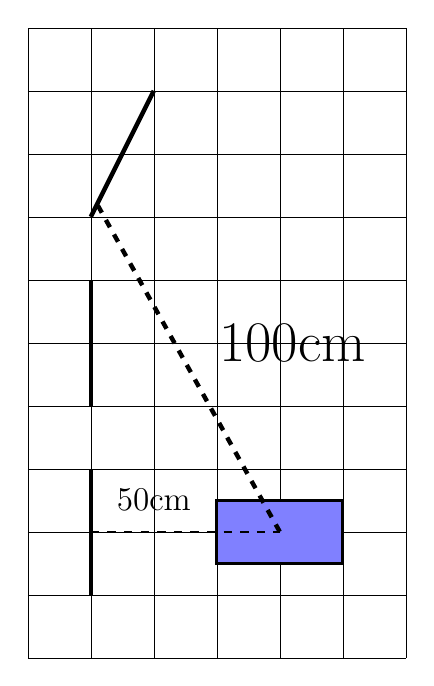
\begin{tikzpicture}[scale=0.8]
			\draw [ultra thin] (0,0) grid (6,10);
			\filldraw[fill=blue!50, very thick] (3,1.5) rectangle (5,2.5);
			\draw [ultra thick] (1,1) -- (1,3);
			\draw [ultra thick] (1,4) -- (1,6);
			\draw [ultra thick] (1,7) -- (2,9);
			\node at (2,2.5) {\large 50cm};
			\draw [dashed, thick] (1,2) -- (4,2);
			\node at (4.2,5) {\huge 100cm};
			\draw [dashed, ultra thick] (4,2) -- (1.1,7.2);

		\end{tikzpicture}
		\caption{センサデータは左前方の一点を利用する}
	\end{minipage}
	\begin{minipage}{0.5\hsize}
		\centering
		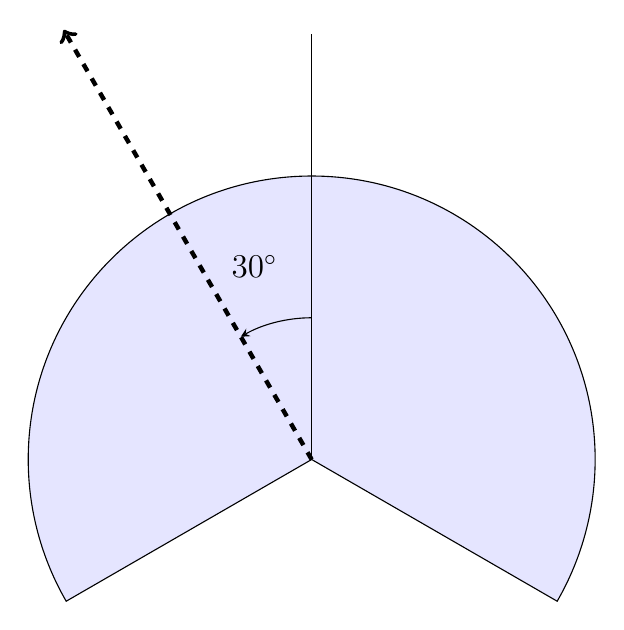
\begin{tikzpicture}[scale=0.9]
			\filldraw[fill=blue!10] (0,0) -- (330:4) arc (330:360:4) arc (0:210:4) --cycle;
			\draw (0,0) -- (90:6);
			\draw[dashed, ultra thick, ->] (0,0) -- (120:7);
			\draw[-stealth] (90:2) arc (90:120:2) node[right] at (115:3){\large $30^\circ$};
		\end{tikzpicture}
		\caption{センサ範囲}
	\end{minipage}
\end{figure}

\begin{figure}[H]
	\begin{minipage}{0.5\hsize}
		\setlength{\parindent}{1\Cwd}
		もやし
	\end{minipage}
	\begin{minipage}{0.5\hsize}
		\centering
		\begin{figure}[H]
			\centering
			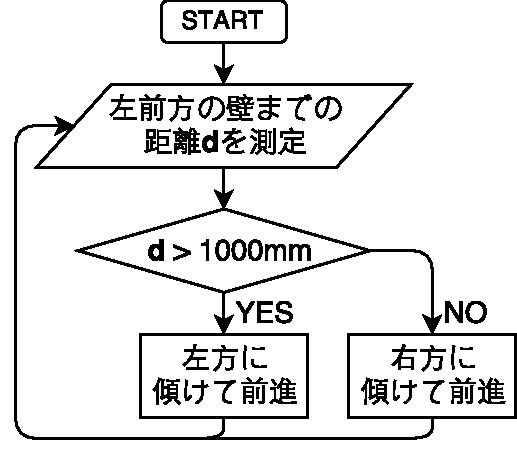
\includegraphics[width=8.5cm]{img/wall_01.pdf}
			\caption{壁並走アルゴリズム案}
		\end{figure}
	\end{minipage}
\end{figure}


\section{結果}
\section{考察}

\end{document}
